\newpage
\section{Implementation}

This part will explain our implementation of VEM for the resolution of Laplace problem with Dirichlet boundary conditions in $2$D and $3$D, on respectively polygonal or polyhedral meshes. C++ has been used, making the most of the fact that it is an object oriented programming language. Moreover, a Makefile has been written to automate compilation, and a Doxygen full documentation of the implementation can also be automatically generated. To visualize the results, we have however preferred to create some Python scripts, taking advantage of Mayavi library for $3$D plots. We have tried to adopt a coding style as coherent and easily readable as possible, to make the comprehension easier. 

\subsection{Global view on the code}
The code is based on $18$ classes and a main file. Making the most of \textit{template programming} techniques, declaration and implementation of each class are both in a header file. Memory layout has been done with the most recent C++ techniques in order to avoid memory leaks. In particular, where pointers are necessary, they have been implemented as smart (shared or weak) pointers. While writing the code, our aim has always been to create a code as general and reusable as possible. The code is essentially and ideally divided into two main parts:
\begin{itemize}
\item \textbf{The mesh:} $7$ classes serve to its implementation, where any $2$D or $3$D mesh composed by non-necessarily convex elements are modelled. The flexibility brought by VEM with respect to the geometry makes this part quite complex and computationally not negligible. Computing some properties of the polygons/polyhedrons (as the elements volume, external normal, etc.) is significantly more complex than for standard grids or triangular meshes, but it is essential for the problem resolution. 
\item \textbf{Problem solving using VEM:} in this part, we have first tried to create a code that solves Laplace problem on any mesh regardless of the type of solver and of the imposed boundary conditions. Based from this first working part, we have implemented the Virtual Element Method solver and Dirichlet boundary conditions, the only solver and boundary conditions considered in this project. The idea has been to implement a code that is as general as possible, so that we could modify the method (for example to use the Finite Element Mehod instead of VEM) by only writing a new class corresponding to a new solver, without touching the part corresponding to the problem or the boundary conditions. In the same way, we could easily add some classes to consider other equations or other boundary conditions. 
\end{itemize}

Apart from those two main parts, there is a \textit{main} file where the appropriate solver can be run. The parameters needed to solve the problem (type of geometry, type of mesh, force term, name of the output file, etc.) are specified in a \textit{datafile} so that we do not need to recompile the whole code for any small modification. 

As already said, we have also added a separate part written in Python in order to have a graphical visualization of the results. Python has been chosen thanks to its simplicity compared to C++ for the implementation of graphical interfaces, and thanks to the presence of the library \textit{Mayavi}, well adapted to $3$D visualization. This has been implemented to be complementary to the rest of the code, in order to furnish a fast way to graphically verify  the solutions. 

\subsection{Mesh}
We have chosen to write from scratch the code to create a mesh because of the particularity of VEM to handle more general elements compared to the classical Finite Element Method. 

A mesh in $3$D has been thought as an ensemble of polyhedrons. Each polyhedron is composed of a set of polygons that are themselves defined as an ordered set of points. The class \verb|Mesh| is based on the $3$ classes that represent polyhedrons, polygons and points. Those three classes are tightly interconnected: each polyhedron contains a vector of pointers to the points corresponding to its vertices, and an other vector of pointers to the polygons corresponding to its faces. This makes the constructor of such objects more difficult to write, but the difficulties have been surmounted thanks to the \textit{variadic template} techniques and to a method fully dedicated to the creation of instances. In this situation, we have also chosen to use \textit{shared pointers} when pointers are needed to make the memory management easier to handle. It has been decided not to use \textit{unique pointers} since inside the program, the same pointer can be used by different instances of different classes. 

A mesh in $2$D has been implemented in a similar way, but avoiding the presence of polyhedrons. However, a class Edge has not been necessary, thus it has not been implemented in order to keep a structure as simple as possible. 

Two template parameters, \textit{embedded} and \textit{real} are present in every class. They guarantee some flexibility with respect to the chosen space ($2$D or $3$D) and to the precision of the data (double or long double types can be used). 

\subsubsection{Point and MeshPoint} \label{pts}
The classes \verb|Point| and \verb|MeshPoint| both represent a point in the $2$D or $3$D space. However, as their names suggest, \verb|Point| represents a generic point while \verb|MeshPoint| represent a point belonging to a mesh. In each instance of \verb|MeshPoint| the polygons and polyhedrons that have this point as vertex are also stored. No copy constructor is implemented in \verb|MeshPoint|, copying any such instance is forbidden. \verb|MeshPoint| also keeps into memory the ID of the point corresponding to the given mesh, and the information about whether a point is on the boundary of the considered geometry or not. 

Class \verb|Point| is also used to represent a (geometrical) vector. Indeed, a point is only represented by an array of numbers corresponding to its coordinates. This is also sufficient to represent a vector. This is why class Point also contains methods to compute the norm of a vector or a cross product. 

The presence or the absence of the copy constructor is however the main difference between both classes: in class Point, it is very useful to compute faster everything we need; but in \verb|MeshPoint| it would even be harmful. Indeed, it would be difficult to keep the tight interconnection between classes used to create meshes if one of their component (as a vertex) were copied. \\

Here is reported the implementation of class \verb|Point| and its main methods: \\


\noindent\rule{12.7cm}{1pt}
\begin{lstlisting}[caption=File \texttt{Point.h}]
template <long embedded,typename real=double>
class Point {

protected:
  array<real,embedded> coordinates;

public:
  // CONSTRUCTORS
  Point(const array<real,embedded>& inputArray);
  Point(const Point<embedded,real>& inputPoint);
  Point(const MeshPoint<embedded,real>& inputPoint);

  // Constructor with variadic template
  template <typename... Args>
  Point(Args... arguments);

  // STANDARD METHODS
  long maxIndex() const;	//!< Maximum index of the point
  long maxAbsIndex() const;	//!< Maximum index of the point with absolute value
  real norm() const;  //!< L2 norm of the vector
  real normL1() const; //!< L1 norm of the vector

  real& operator[](long index);	//!< Get an element by reference

  template <long embedded2,typename real2>
  friend Point<embedded2,real2> cross(const Point<embedded2,
real2>& point1, const Point<embedded2,real2>& point2);
};
\end{lstlisting}

\noindent\rule{12.7cm}{1pt}\\

Here is reported the implementation of class \verb|MeshPoint| and its main methods:\\

\noindent\rule{12.7cm}{1pt}
\begin{lstlisting}[caption=File \texttt{MeshPoint.h}]
template <long embedded,typename real=double>
class MeshPoint: public Point<embedded,real> {
protected:
  // PROPERTIES
  long pointID;	//!< ID of the MeshPoint
  real value;		//!< Value in the point after the resolution of the problem
  bool isBoundary;	//<! Tells if the MeshPoint is on the boundary

  vector<weak_ptr<Polygon<embedded, real>>> polygonVector;
  vector<weak_ptr<Polyhedron<embedded,real>>> polyhedronVector;

  // CONSTRUCTORS
  // Constructor with variadic template
  template <typename... Args>
  MeshPoint(Args... arguments);

  // STANDARD METHODS
  void addPolygon(weak_ptr<Polygon<embedded,real>> 
inputPolygon); //!< It inserts in polygon vector a new Polygon
  void addPolyhedron(weak_ptr<Polyhedron<embedded,real>> 
inputPolyhedron); //!< It insert in polyhedron vector a new Polyhedron
\end{lstlisting}

\noindent\rule{12.7cm}{1pt}\\

\subsubsection{Polygon and Polyhedron}
The two classes \verb|Polygon| and \verb|Polyhedron| represent a generic polygon or polyhedron, not necessarily convex. Both classes are to be understood as mesh components; but we have not implemented two different classes of both as for Point since it has not been necessary. The absence of copy constructor is then required as for \verb|MeshPoint|, for the same reasons (see paragraph \ref{pts}). For both classes \verb|Polygon| and \verb|Polyhedron|, the only way to create a new instance is by using methods \verb|make_shared_Polygon| or \verb|make_shared_Polyhedron|, that return a shared pointer to the new instance and that take care of handling connexions between them (since they are components of a given mesh). 
The use of \textit{variadic template} techniques guarantee some flexibility and readability of the code. For example, a \verb|Polygon| can be initialized either from an \verb|std::vector| of \verb|MeshPoint|s, or from an arbitrary number of \verb|MeshPoint|s. 

\verb|Polygon| is modelled as an ordered set of \verb|Point|s, in $2$D or $3$D. The order is necessary in order to be able to determine the sense of a normal vector, and in order to know if a polygon is convex or not (see paragraph \ref{polygons}). During the instantiation, the area, the normal vector and the barycenter of the polygon are computed. \verb|Polyhedron| instead, is a non ordered set of \verb|Polygon|s (see paragraph \ref{polyhedron}). During the instantiation are computed the volume, the external normal and the barycenter, and the normal vectors of the faces are coherently oriented (see paragraph \ref{polyhedron} for the algorithms used). \\

Here is reported the implementation of class \verb|Polygon| and its main methods:\\

\noindent\rule{12.7cm}{1pt}
\begin{lstlisting}[caption=File \texttt{Polygon.h}]
template <long embedded, typename real=double>
class Polygon: public std::enable_shared_from_this<Polygon<
embedded,real>> {
protected:
  // PROPERTIES
  // Vector of ordered vertexes
  vector<shared_ptr<MeshPoint<embedded,real>>> pointVector;
	
  bool isBoundary;	// Tells if the Polygon is on the boundary
  real area;	// \return the area of the Polygon
  Vector<3, real> normal;	// oriented normal to the Polygon
  Point<embedded, real> centroid;	// centroid of the Polygon
  vector<weak_ptr<Polyhedron<embedded,real>>> polyhedronVector;

public:
  // CONSTRUCTORS
  Polygon(const privateStruct &, const vector<shared_ptr<
MeshPoint<embedded,real>>>& vertexVector);
  // Constructor with variadic template.
  template <typename... Args>
  Polygon(const privateStruct&,Args... arguments);

  template <typename... Args>
  static shared_ptr<Polygon<embedded,real>> make_shared_Polygon
(Args... arguments);

public:
  // STANDARD METHODS
  // Add a new vertex to the Polygon
  void addPoint(const shared_ptr<MeshPoint<embedded,real>>& p1); 
  // Add a new Polyhedron having this as face
  void addPolyhedron(weak_ptr<Polyhedron<embedded,real>> 
polyhedron);	
			
  Vector<embedded,real> computeCentroid();
  real computeArea();
  real getDiameter();
  real hTriangle(); // Compute the maximum distance between 2 vertexes.

  shared_ptr<MeshPoint<embedded,real>> isPointAVertex(Point
<embedded,real>& point);	
  bool isPointInside(Point<embedded,real>& point);
  array<shared_ptr<MeshPoint<embedded,real>>,2> 
isPointOnBoundary(Point<embedded,real>& point);

  Vector<3,real> computeNormal();
  void switchPointsOrder(); // Invert the orientation of the Polygon
\end{lstlisting}

\noindent\rule{12.7cm}{1pt}\\

Here is reported the implementation of class \verb|Polyhedron| and its main methods:

\noindent\rule{12.7cm}{1pt}
\begin{lstlisting}[caption=File \texttt{Polyhedron.h}]
template <long embedded, typename real=double>
class Polyhedron: public enable_shared_from_this<Polyhedron
<embedded,real>> {

protected:
  // PROPERTIES
  // Stores the faces of the Polyhedron
  vector<shared_ptr<Polygon<embedded,real>>> polygonVector; 
	
  bool isBoundary;	// Tells if the Polygon is on the boundary
  real volume;	// volume of the Polyhedron
  Point<embedded,real> centroid;	// Not the real centroid, only the mean of the vertexes.

  // Stores the vertexes of the Polyhedron
  vector<shared_ptr<MeshPoint<embedded,real>>> pointVector;	

public:
  // CONSTRUCTORS
  Polyhedron(const privateStruct&,const vector<shared_ptr
<Polygon<embedded,real>>>& inputPolygonVector);
  // Constructor with variadic template. DO NOT USE.
  template <typename... Args>
  Polyhedron(const privateStruct&,Args... arguments)

  template <typename ...Args>
  static shared_ptr<Polyhedron<embedded, real>>
make_shared_Polyhedron;

  // STANDARD METHODS
  // Add a new vertex to the Polygon
  void addPolygon(shared_ptr<Polygon<embedded,real>>& 
inputPolygon);
  // Add a new Polyhedron having this as face
  void addPoint(shared_ptr<MeshPoint<embedded,real>>& 
inputPoint);
  Point<embedded,real> computeCentroid();	// return the centroid
  real computeVolume();	// return the volume of the Polyhedron
  real getDiameter();		// return the maximum distance between 2 Points
  // Makes the normal to each face pointing towards the external of the Polyhedron
  void fixExternalNormal();	
  // Makes the normal of each face pointing in the same direction (or inward or outward)
  void fixFacesOrientation();	
  // Maximum distance between vertexes. Necessary for the mesh.
  real hTriangle();	
  void linkPoints();	// Makes all vertexes pointing to this
  void linkPolygons();  // Makes all Polygons pointing to this

  void switchFacesOrientation();	// Invert the orientation of all faces
  // If a new face is added, also his vertexes are added to the pointVector
  void updatePointVector();
\end{lstlisting}
\noindent\rule{12.7cm}{1pt}\\

\subsubsection{Mesh, Mesh2D, Mesh3D}
\verb|Mesh| is an abstract class that represents a very general mesh (a solid in a $3$D space, a surface in a $2$D or in a $3$D space, etc.). In each instance of this class are memorized two vectors: one vector of \verb|Point|s and one of \verb|Polygon|s or \verb|Polyhedron|s depending on the chosen space. Basic methods are declared to read different types of files and build the mesh from them; they will suitably be implemented on the derived classes. Two other dedicated virtual methods are also declared in this class to keep track of the boundary elements and to eventually set other mesh properties. A constructor has also been defined and will be automatically called from the constructors of the derived classes. 

\verb|Mesh2D| is a derived class of \verb|Mesh|, used to model $2$D meshes in a $2$D space. For the lifting of the boundary elements, we look for edges present only in a unique polygon of the mesh. To optimize the computational time of research of boundary elements, we have introduced a vector of point tuples called \verb|pairVector|. This allows us to avoid the introduction of a class representing the edges, that would just have made the code uselessly more complex. Once created the mesh, \verb|pairVector| is analysed to find non duplicated edges. 

\verb|Mesh3D| is similar to \verb|Mesh2D| but to model $3$D meshes in a $3$D space. Because of the higher complexity of the mesh, it has been decided to also save the pointers to the faces of the polygon into a vector. This has allowed us to obtain the boundary elements with a similar algorithm to the $2$D case, but comparing the faces instead of the edges. In this case, and to make it faster, the algorithm to compare the faces is directly called at the instantiation of every new face. \\

Here is reported the implementation of class \verb|Mesh| and its main methods:

\noindent\rule{12.7cm}{1pt}
\begin{lstlisting}[caption=File \texttt{Mesh.h}]
template <long embedded,typename baseElement,OpenEnum isOpen=
OPEN, typename real=double>
class Mesh {
protected:
    
    // Vector of Polygon or Polyhedron
    vector<shared_ptr<baseElement>> elementVector;	
    // Vector of the vertexes of each element
    vector<shared_ptr<MeshPoint<embedded,real>>> pointVector;	
	
public:
    long numberOfElements;
    long numberOfPoints;

    virtual real hTriangle();	// paramether h of the Mesh
	
    // Method that calls the functions that read the file
    void initialize(string pointFile,string connection,
MeshType meshType=ANYTHING3D);

    // It obtains the pointVector from file
    virtual void setPointVector(string file);	
    // It obtains the elementVector from connections
    virtual void setElementVector(string connections, MeshType
meshType);
    
    // Virtual method to keep into account the boundary 
elements
    virtual void setBoundaryElements()=0;
    //	Virtual method used to set other things, like pointIDs
    virtual void setRemainingThings()=0;

    // methods to set the elementVector
    virtual void setTetrahedronMesh(string connection); 
    virtual void setTriangleMesh(string connection);	
    virtual void setAnything3DMesh(string connection);
    virtual void setAnything2DMesh(string connection);
    virtual void setFileType1Mesh(string connection);
    virtual void setFileType2Mesh(string connection);

    virtual void sort(); //!< Sort the pointVector based on pointID
\end{lstlisting}

\noindent\rule{12.7cm}{1pt}\\

Here is reported the implementation of class \verb|Mesh2D| and its main methods:

\noindent\rule{12.7cm}{1pt}
\begin{lstlisting}[caption=File \texttt{Mesh2D.h}]
template <typename real=double>
class Mesh2D: public Mesh<2,Polygon<2,real>,OPEN,real> {
private:
    // This is to obtain internal and external points	
    vector<pair<long,long>> pairVector;

public:
    long numberOfBoundaryPoints;
	
    // Constructor with input file
    Mesh2D(string pointFile,string connectionFile,MeshType 
meshType=ANYTHING2D);

    template <typename... Args >
    shared_ptr<Polygon<2,real>> newPolygon(Args... arguments);

    // Mesh of ANYTHING2D type
    virtual void setAnything2DMesh(string connection);

    virtual void setBoundaryElements();
    virtual void setRemainingThings();
\end{lstlisting}
\noindent\rule{12.7cm}{1pt}\\

Here is reported the implementation of class \verb|Mesh3D| and its main methods:

\noindent\rule{12.7cm}{1pt}
\begin{lstlisting}[caption=File \texttt{Mesh3D.h}]
template <typename real=double>
class Mesh3D : public Mesh<3, Polyhedron<3,real>, OPEN, real> {
protected:
    // Vector of all the Polyhedron faces
    vector<shared_ptr<Polygon<3,real>>> polygonVector;  

public:
    long numberOfPolygons;
    long numberOfBoundaryPoints;

    // Constructor with input file
    Mesh3D(string pointFile,string connectionFile,MeshType 
meshType=ANYTHING3D);
	
    // STANDARD METHODS
    // Method to create a Polygon after having read it.
    template <typename... Args >
    shared_ptr<Polygon<3,real>> newFace(Args... arguments);

    virtual void setBoundaryElements();
    virtual void setRemainingThings();

    // Mesh of TETRAHEDRON type
    virtual void setTetrahedronMesh(string connection);
    // Mesh of ANYTHING3D type
    virtual void setAnything3DMesh(string connection);
\end{lstlisting}
\noindent\rule{12.7cm}{1pt}\\

\subsection{Laplace equation and VEM solver}
For the part of the code that solves a numerical problem, we have tried to write a code as modular as possible, to be able to change solver easily or to consider different boundary conditions (even if in this project, only VEM and Dirichlet boundary conditions have been implemented). We have deeply use \textit{template programming} techniques to guarantee this modularity. Indeed, classes that model the numerical problem are all template classes, for which two parameters are needed: one for the type of solver, \verb|SolverType|, and one for the boundary conditions, \verb|BoundaryConditionType|. A last class has been implemented to compute the error. To manage matrices, vectors and linear systems, the open-source Eigen library has been used. 

\subsubsection{Problem and Laplace classes}
The abstract class \verb|Problem| models a very generic numerical problem, that can be solved through a linear system made of a stiffness matrix and of a forcing term. The aim of class \verb|Problem| is to define a common interface for all types of problems, containing the definition of all the necessary methods and the implementation of the most generic ones. In particular, the creating {\color{red} creation?} of the stiffness matrix and of the forcing term are left to the derived classes while a default linear system solver is implemented in the parent class (BiCGSTAB) that can be overwritten. In \verb|Problem| are also implemented methods to compute the error and to write the output on a file, since this is common to all the solvers. 

\verb|Laplace| is a class that inherits from \verb|Problem| in order to model Laplace problems, leaving the full choice of the type of solver and of appropriate boundary conditions, as discussed earlier. In this class are implemented the methods to assemble the linear system and the global stiffness matrix, even if it leaves the computation of the local stiffness matrix to the classes dedicated to the solver and to the boundary conditions. \\

Here is reported the implementation of class \verb|Problem| and its main methods:

\noindent\rule{12.7cm}{1pt}
\begin{lstlisting}[caption=File \texttt{Problem.h}]
template <long embedded,typename MeshType,typename real=double>
class Problem {
	
protected:
    const MeshType& mesh;	//!< Mesh on which the problem is based

public:
    SparseMatrix<real> stiffnessMatrix;
    VectorX<real> knownTerm;
    VectorX<real> solution;
	
public:
    // General constructor for the Problem
    Problem(const MeshType& inputMesh)

    // Virtual method to compute the stiffness matrix
    virtual void computeStiffnessMatrix()=0;
    // Virtual method to compute the known term
    virtual void computeKnownTerm()=0;	

    virtual void computeSolution();
    virtual void operator()();  // Method to execute the method.
FreeFem style.

    //  It displays the error after the computation
    virtual void displayError(std::function<real(Point<embedded,
real>&)>
 realSolutionFunction);
    // full output to file 
    virtual void write(string outputPoints,string 
outputConnections,
string outputSolution);	
    // Output to file of the solution
    virtual void writeSolution(string outputSolution="solution.
sol");
\end{lstlisting}
\noindent\rule{12.7cm}{1pt}\\

Here is reported the implementation of class \verb|Laplace| and its main methods:

\noindent\rule{12.7cm}{1pt}

\begin{lstlisting}[caption=File \texttt{Laplace.h}]
template <long embedded,typename MeshType,typename SolverType,
typename BoundaryConditionType,typename real=double>
class Laplace: public Problem<embedded,MeshType,real> {
private:
    real diffusionCoeff;	
public:
    // Vector used to fast build the stifnessMatrix.
    vector<Triplet<real>> tripletList; 
    BoundaryConditionType boundaryCondition;
    SolverType solver;

    // Standard constructor
    Laplace(const MeshType& inputMesh,std::function<real(const 
Point<embedded,real>&)> inputForceTerm,std::function<real(const 
Point<embedded,real>&)> 
inputBoundaryFunction,real inputDiffusionCoeff=1)

    // General method. It invokes the methods of the Solver.
    void computeStiffnessMatrix();
    // General method. It invokes the methods of the Solver and BoundaryCondition 
    void computeKnownTerm();
\end{lstlisting}
\noindent\rule{12.7cm}{1pt}\\

\subsubsection{Monomials and MonomialsPolygon}
First, we recall some VEM theory for a better comprehension. Given a mesh element, we call monomial $m_\alpha$ of degree $|\alpha|$ the following quantity:
$$
m_\alpha:=\bigg( \frac{\mathbf{x}-\mathbf{x_k}}{h_k} \bigg) ^\alpha,
$$
where $\mathbf{x_k}$ is the barycenter of the element, and $h_k$ its diameter. For VEM solver of degree $1$, it is necessary to evaluate the monomials at the vertices of the elements, and to compute their gradients on the elements. 
We note that for VEM of order $1$, neither $\mathbf{x_k}$ nor $h_k$ have to be exactly computed as far as the same values are used to compute all the monomials of a same element. Consequently, it has not been necessary to implement the computation of the exact barycenter of an element, operation computationally very expensive. 
All of this has been implemented in class \verb|Monomials| for the case in which a $2$D (resp. $3$D) element is embedded in a $2$D (resp. $3$D) space.

Class \verb|MonomialsPolygon|, that inherits from  \verb|Monomials|, however, is used to compute the same quantities but in the case where a $2$D element (a polygon) is embedded in a $3$D space. The main difference comes from the fact that in the case of a $2$D (resp. $3$D) element in a $2$D (resp. $3$D) space, the gradient is a vector whose components are all equal, while for a $2$D element in a $3$D space the gradient has to be projected on the plane of the polygon we are considering.\\

Here is reported the implementation of class \verb|Monomials| and its main methods:

\noindent\rule{12.7cm}{1pt}
\begin{lstlisting}[caption=File \texttt{Monomials.h}]
template <long embedded,typename baseElement,typename real=
double>
class Monomials {
public:
    const shared_ptr<baseElement>& element;	//!< Element can be Polygon or Polyhedron
    real diameter;  //!< Diameter of the element
    Point<embedded,real> centroid;  //!< Centroid of the element
    // It's the gradient of the monomial. It's 1/diameter
    real gradient;

    // CONSTRUCTOR
    Monomials(const shared_ptr<baseElement>& figure);

    // Function to evaluate the monomial in a point
    real evaluate (const Point<embedded,real>& p, long i);
}
\end{lstlisting}
\noindent\rule{12.7cm}{1pt}\\

Here is reported the implementation of class \verb|MonomialsPolygon| and its main methods:

\noindent\rule{12.7cm}{1pt}
\begin{lstlisting}[caption=File \texttt{MonomialsPolygon.h}]
template <typename real>
class MonomialsPolygon: public Monomials<3, Polygon<3,real>,
real> {
public:
    // these are virtual indexes used to project the Polygon on an appropriate plane
    long indexX;
    long indexY;
    long indexZ;
    Vector<3,real> gradientX;
    Vector<3,real> gradientY;
	
    MonomialsPolygon(const shared_ptr<Polygon<3,real>>& figure); 
    
    // Function to evaluate the monomial in a point
    real evaluate (const Point<3,real>& p, long i);
\end{lstlisting}

\noindent\rule{12.7cm}{1pt}\\

\subsubsection{Solver, SolverVEM, SolverVEM2D and SolverVEM3D}
Class \verb|Solver| and its inherited classes contain the implementation of the numerical solvers. Concerning the VEM solver, we refer to chapter \ref{theory} for the description of the method, but we will give in this paragraph a description of its implementation. 

\verb|Solver| is an abstract class that represents a generic solver. Only one method is present in this class, \verb|computeLocalK|, whose aim is to compute the local stiffness matrix. It is consequently a class that can be extended to any numerical method that need the computation of a local stiffness matrix on every element. 

To implement the VEM solver, it has not been possible to create a unique class for the $2$D and the $3$D cases. As a consequence, a generic abstract class \verb|SolverVEM| has been created and directly inherits from \verb|Solver|, while \verb|SolverVEM2D| and \verb|SolverVEM3D| inherit from \verb|SolverVEM|. In \verb|SolverVEM| are implemented the methods that are common to the $2$D and the $3$D cases, while in the lower-level classes are implemented the few specific methods left. 

The VEM solver follows the procedure explained in the article \textbf{TODO REFERENCE!!!!!!}, where matrices $G$, $B$, $D$, $\Pi_\star^\Delta,\Pi^\Delta$ need to be computed in order to then be able to get the local matrix:
$$ \mathbf{K_E^h= (\Pi^\Delta_\star)^T \tilde{G}
  (\Pi^\Delta_\star)+(I-\Pi^\Delta)^T (I-\Pi^\Delta)}. $$ 
Classes \verb|Monomials| and \verb|MonomialsPolygon| have also been used to evaluate the monomials, characteristic of the virtual elements method. Computing $B$ and the forcing term has been left to the lower-level classes while the rest has been implemented in \verb|SolverVEM|. The $3$D case has required a more complex evaluation of boundary terms. Computing the interpolating VEM polynomial on every face has also been necessary, and this operation considerably increases the computational time. 

An important matrix property of VEM is the identity $G = BD$, which is very useful to test the code. A control has thus been implemented in order to tell the user if this identity is not verified. We have indeed tested the code thanks to this identity, also on very particular geometries, such as the one showed in Figure \ref{geom}. \\

Here is reported the implementation of class \verb|Solver| and its main methods:

\noindent\rule{12.7cm}{1pt}
\begin{lstlisting}[caption=File \texttt{Solver.h}]
template <long embedded,typename baseElement,typename 
MatrixType,typename real>
class Solver {
protected:
    std::function<real(const Point<embedded,real>&)> forceTerm;
	
public:
    Solver(std::function<real(const Point<embedded,real>&)> 
inputForceTerm);

    // Main virtual method. To be implemented in subclasses
    virtual MatrixType computeLocalK(const shared_ptr
<baseElement>& element)=0;
};
\end{lstlisting}

\noindent\rule{12.7cm}{1pt}\\

Here is reported the implementation of class \verb|SolverVEM| and its main methods:

\noindent\rule{12.7cm}{1pt}
\begin{lstlisting}[caption=File \texttt{SolverVEM.h}]
template <long embedded,long elementDimension,typename 
baseElement, typename MonomialType,typename real=double>
class SolverVEM: public Solver<embedded,baseElement,
Matrix<real,Dynamic,Dynamic>,real> {

protected:
    virtual Matrix<real,elementDimension+1,elementDimension
+1> computeG(MonomialType& monomial);

    virtual Matrix<real,elementDimension+1,Dynamic> 
computeB(const shared_ptr<baseElement>& polyhedron,
MonomialType& monomial)=0;

    virtual Matrix<real,Dynamic,elementDimension+1> 
computeD(MonomialType& monomial);
	
    virtual Matrix<real,elementDimension+1,Dynamic> 
computePIStar(
Matrix<real,elementDimension+1,elementDimension+1>&G,
Matrix<real,elementDimension+1,Dynamic>&B);

    virtual Matrix<real,Dynamic,Dynamic> computePI(
Matrix<real,elementDimension+1,Dynamic>&PIStar,
Matrix<real,Dynamic,elementDimension+1>&D);
	
public:
    //Basic constructor. A lot of paramethers are given as template.
    SolverVEM(std::function<real(const Point<embedded,real>&)>
inputForceTerm);
	
    // This is to compute the local stiffness matrix
    virtual Matrix<real,Dynamic,Dynamic> computeLocalK(const
shared_ptr<baseElement>& element); 
    //!< Virtual method to compute the known term.
    virtual real computeKnownTerm(const shared_ptr<baseElement>& 
element, const shared_ptr<MeshPoint<embedded,real>>& point)=0; 
};
\end{lstlisting}

\noindent\rule{12.7cm}{1pt}\\

Here is reported the implementation of class \verb|SolverVEM2D| and its main methods:

\noindent\rule{12.7cm}{1pt}
\begin{lstlisting}[caption=File \texttt{SolverVEM2D.h}]
template <typename real=double>
class SolverVEM2D: public SolverVEM<2,2,Polygon<2,real>,
Monomial2D<real>,real> {
public:
    virtual Matrix<real,3,Dynamic> computeB(const shared_ptr
<Polygon<2,real>>& polygon,Monomial2D<real>& monomial);

public:
     SolverVEM2D(std::function<real(const Point<2,real>&)> 
inputForceTerm);
    
     virtual real computeKnownTerm(const shared_ptr<Polygon<2,
real>>& element,
const shared_ptr<MeshPoint<2,real>>& point);
};
\end{lstlisting}

\noindent\rule{12.7cm}{1pt}\\

Here is reported the implementation of class \verb|SolverVEM3D| and its main methods:

\noindent\rule{12.7cm}{1pt}
\begin{lstlisting}[caption=File \texttt{SolverVEM3D.h}]
template <typename real=double>
class SolverVEM3D: public SolverVEM<3,3,Polyhedron<3,real>,
Monomial3D<real>,real> {
public:
    virtual Matrix<real,3,3> computeGPolygon(MonomialsPolygon
<real>& monomial);
    virtual Matrix<real,4,Dynamic> computeB(const shared_ptr
<Polyhedron<3,real>>& 
polyhedron,Monomial3D<real>& monomial);

    virtual Matrix<real,3,Dynamic> computeBPolygon(const 
shared_ptr<Polygon<3,real>>& 
polyhedron,MonomialsPolygon<real>& monomial);

    virtual Matrix<real,Dynamic,3> computeDPolygon(
MonomialsPolygon<real>& monomial);
		
    virtual Matrix<real,3,Dynamic> computePIStarPolygon(Matrix
<real,3,3>&G, Matrix<real,3,Dynamic>&B);
	
public:
    SolverVEM3D(std::function<real(const Point<3,real>&)> 
inputForceTerm);
 
    virtual real computeKnownTerm(const shared_ptr<Polyhedron
<3, real>>& element, const shared_ptr<MeshPoint<3,real>>& 
point);	
};

\end{lstlisting}
\noindent\rule{12.7cm}{1pt}\\

\subsubsection{BoundaryCondition, Dirichlet}
Class \verb|BoundaryCondition| is an abstract class that represents any type of boundary conditions and handle them. Class \verb|Dirichlet| inherits from \verb|BoundaryCondition| and takes only care of Dirichlet boundary conditions, as its name suggests. To impose this type of condition, the upper-left block of the stiffness matrix (whose rows correspond to boundary elements) needs to be diagonal. Moreover, the same rows corresponding to the boundary elements in the forcing term need to be correctly set. 

Those two classes are based on the three following main methods: 
\begin{itemize}
\item Process the local stiffness matrix before assembling the global stiffness matrix. In the Dirichlet case, if an element is on the boundary, its local stiffness matrix is not assembled with the other ones in order to keep the upper-left block of the global stiffness matrix diagonal. 
\item Process the global stiffness matrix after its assembling. In the Dirichlet case, we make sure that the upper-left block is diagonal. 
\item Process the forcing term after it has been created, that is we set correctly the rows corresponding to the boundary elements. 
\end{itemize}

Here is reported the implementation of class \verb|BoundaryCondition| and its main methods:

\noindent\rule{12.7cm}{1pt}
\begin{lstlisting}[caption=File \texttt{BoundaryCondition.h}]
template <long embedded,typename MeshType,typename MeshElement,
typename real=double>
class BoundaryCondition {
protected:
    const MeshType& mesh;
    std::function<real(Point<embedded,real>&)> boundaryFunction;

    BoundaryCondition(const MeshType&
inputMesh,std::function<real(Point<embedded,real>&)> 
inputBoundaryFunction);

public:
    // This is to decide if to add the Kloc computed to the matrix
    virtual void addToTripletList(Matrix<real,Dynamic,
Dynamic>& Kloc, MeshElement& element,vector<Triplet<real>>& 
tripletList)=0;
	
    // Changes the stiffnessMatrix to keep into account the boundary condition.
    virtual void assignBoundaryConditionOnStiffnessMatrix
(vector<Triplet<real>>& tripletList)=0;
	
    // Changes the known term to keep into account the boundary condition
    virtual void assignBoundaryConditionOnKnownTerm
(VectorX<real>& knownTerm)=0; 		
};

\end{lstlisting}

\noindent\rule{12.7cm}{1pt}\\

Here is reported the implementation of class \verb|Dirichlet| and its main methods:

\noindent\rule{12.7cm}{1pt}
\begin{lstlisting}[caption=File \texttt{Dirichlet.h}]
template <long embedded,typename MeshType,typename MeshElement,
typename real>
class Dirichlet: public BoundaryCondition<embedded,MeshType,
MeshElement,real> {
    long numberOfPoints;
    long numberOfBoundaryPoints;

public:
    // Standard constructor
    Dirichlet(const MeshType& mesh,std::function<real(Point
<embedded,real>&)> boundaryFunction);
	
    // This is to decide if to add the Kloc computed to the matrix.
    virtual void addToTripletList(Matrix<real,Dynamic,Dynamic>& 
Kloc, MeshElement& element,vector<Triplet<real>>& tripletList);
	
    // Changes the stiffnessMatrix to keep into account the boundary condition.
    virtual void assignBoundaryConditionOnStiffnessMatrix
(vector<Triplet<real>>& tripletList);
	
    // Changes the known term to keep into account the boundary condition
    virtual void assignBoundaryConditionOnKnownTerm(VectorX
<real>& knownTerm);	
};

template <typename real=double>
using Dirichlet3D=Dirichlet<3,Mesh3D<real>,Polyhedron<3,real>,
real>;

template <typename real=double>
using Dirichlet2D=Dirichlet<2,Mesh2D<real>,Polygon<2,real>,
real>;
\end{lstlisting}
\noindent\rule{12.7cm}{1pt}\\

\subsubsection{Error}
\verb|Error| is a class reserved for error computation. The error is computed in two different ways:
\begin{itemize}
\item $l^\infty$ norm: the maximum between the exact and the numerical solution in the nodes;
\item $H^1$ discrete norm: computed as $u^TKu$, where $u$ is the difference between the real and the numerical solutions on the nodes, and $K$ is the stiffness matrix. 
\end{itemize}

Here is reported the implementation of class \verb|Error| and its main methods:

\noindent\rule{12.7cm}{1pt}
\begin{lstlisting}[caption=File \texttt{Error.h}]
template <long embedded,typename real=double>
class Error {
protected:
    const VectorX<real>& solution;
    VectorX<real> realSolution;
    VectorX<real> difference;
    const vector<shared_ptr<MeshPoint<embedded,real>>>& 
pointVector;
    std::function<real(Point<embedded,real>&)> 
realSolutionFunction;
	
    SparseMatrix<real>& stiffnessMatrix;
	
    // This computes the exact solution, from realSolutionFunction
    void computeRealSolution(); 
	
public:
    Error(const VectorX<real>& inputSolution,
const vector<shared_ptr<MeshPoint<embedded,real>>>& 
inputPointVector,
std::function<real(Point<embedded,real>&)> 
inputRealSolutionFunction,
SparseMatrix<real>& inputStiffnessMatrix);

    // L infinite norm of the error
    real LInfinity();
	
    // H1 discrete norm of the error
    real H1Discrete();
	
    void displayError();   //!< Print the computer error	
};
\end{lstlisting}
\noindent\rule{12.7cm}{1pt}\\

\newpage
\section{Results}

\subsection{Visualization of the results}
For the visualization of the results, we have decided to use the Python programming language instead of C++ thanks to a great choice of libraries. This part is divided into two parts, depending on the used libraries:
\begin{itemize}
\item With {\color{red} the} Matplotlib library, we have created $2$ scripts for the $3$D visualization of either a polyhedron or an entire mesh. The main goal of this script is mainly to test the code; it has not been optimized and thus it might be very slow for large meshes. It is however efficient for smaller mesh and allows us to have a quick visual feedback on the results and their coherence. 
\item With {\color{red} the} Mayavi library, we have create $3$ scripts to visualize the solution. \verb|plotPoints3D| only shows the vertices of the polyhedrons that are part of the mesh, together with the solution at these points. \verb|plot2D| and \verb|plot3D|, instead, show the solution on the whole mesh. In the $3$D case, Mayavi visualization tools can be used to see the solution in different part of the mesh, such as on a section of the mesh for instance. 
\end{itemize}

In the following Figures $1$ to $5$, we show some of the visual results that have been obtained:

\begin{figure}[!h]
\label{img:matplotlibPolyhedron}
\centering
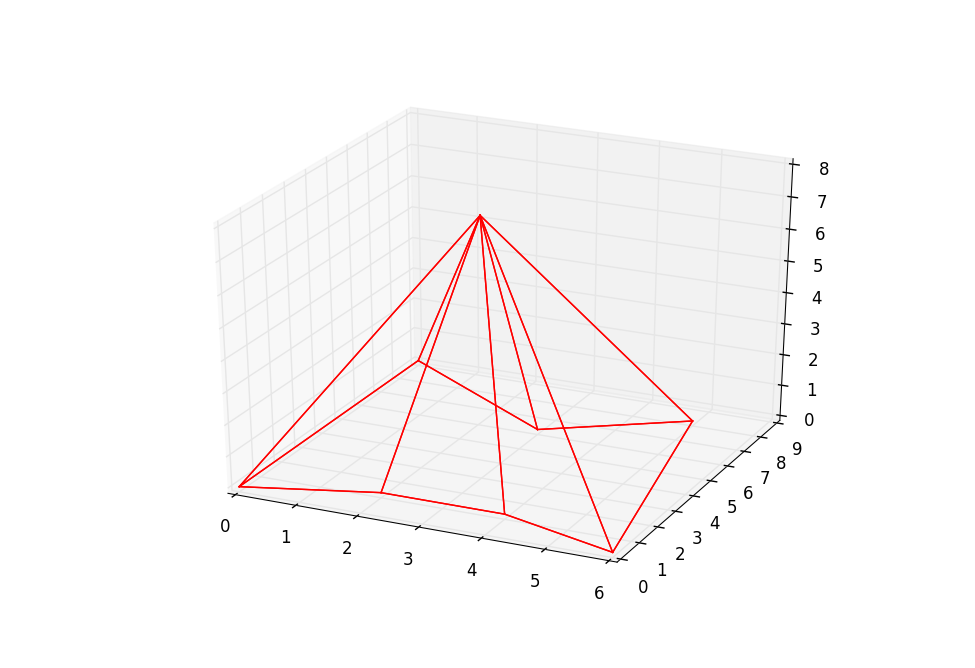
\includegraphics[scale=0.4]{images/matplotlibTest5.png}\label{geom}
\caption{Plot with Matplotlib. A specific mesh element that VEM can handle.}
\end{figure}

\begin{figure}[!h]
\label{img:matplotlibMesh}
\centering
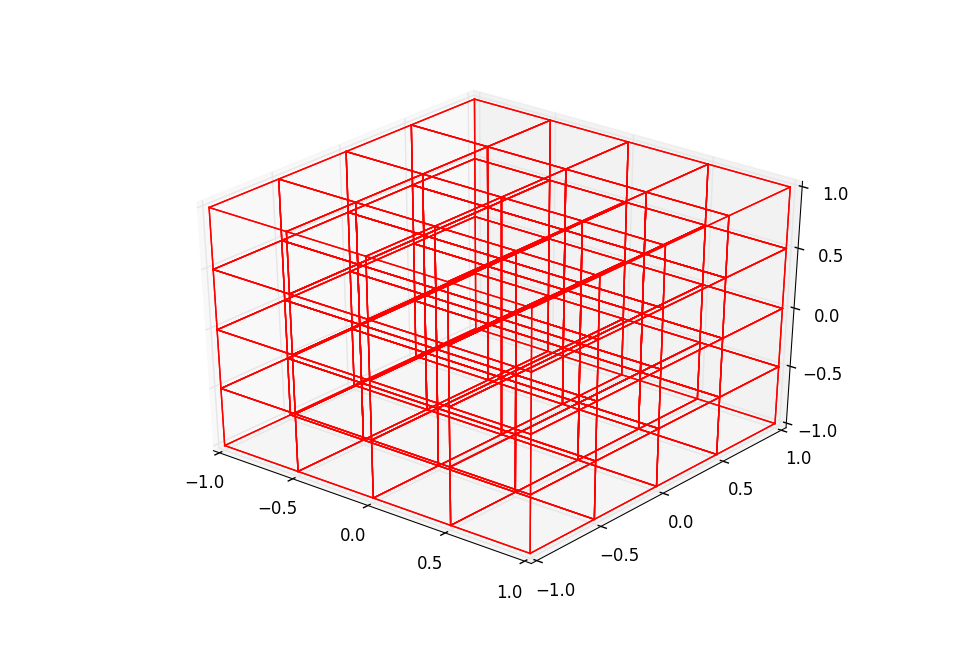
\includegraphics[scale=0.4]{images/matplotlibPlotMesh.png}
\caption{Plot with Matplotlib. Cubic mesh.}
\end{figure}

\begin{figure}[!h]
\label{img:mayavi2D}
\centering
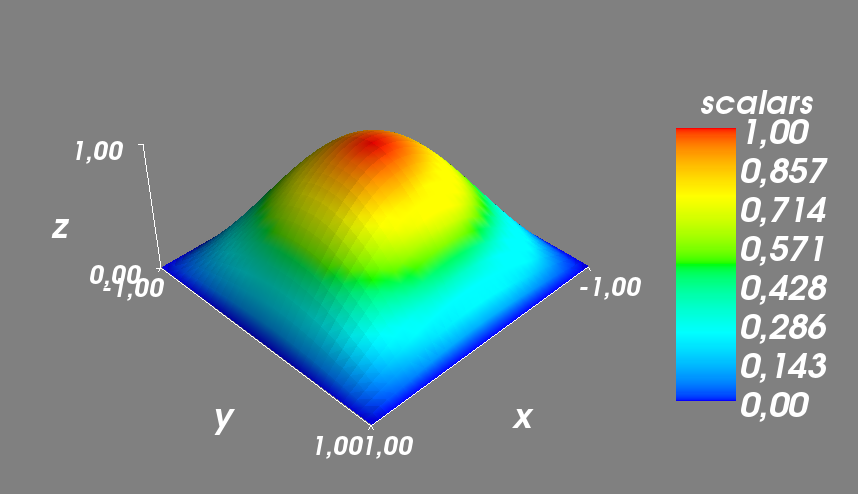
\includegraphics[scale=0.35]{images/mayavi2D.png}
\caption{Plot with Mayavi. $2$D grid mesh with solution.}
\end{figure}

\begin{figure}[!h]
\label{img:matplotlibMesh}
\centering
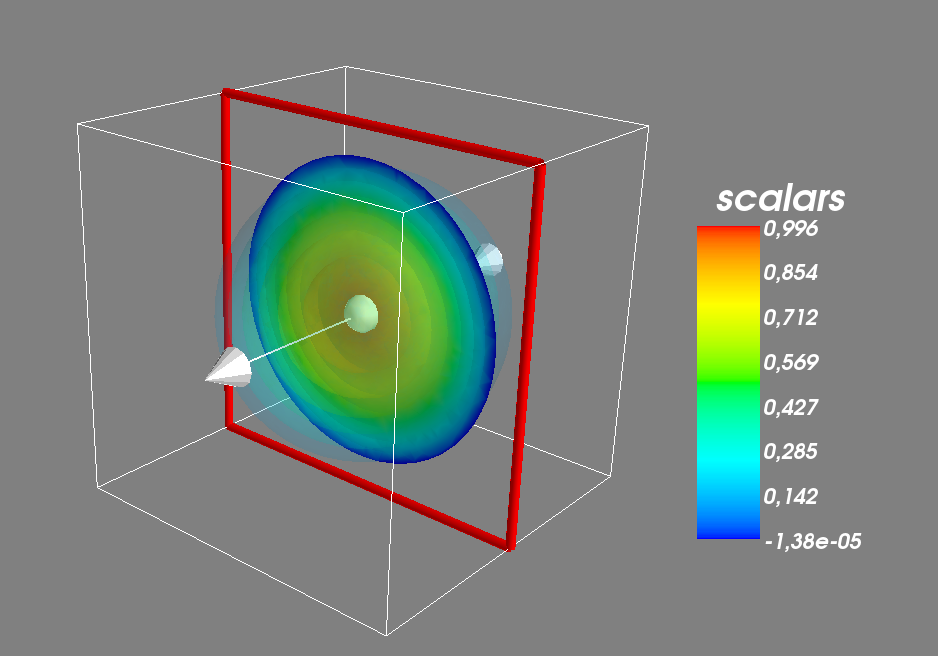
\includegraphics[scale=0.35]{images/mayavi3D.png}
\caption{Plot with Mayavi. Mesh of a tetrahedron on a $3$D sphere with the solution on a section of the sphere. The section can be dynamically chosen.}
\end{figure}

\begin{figure}[!h]
\label{img:matplotlibMesh}
\centering
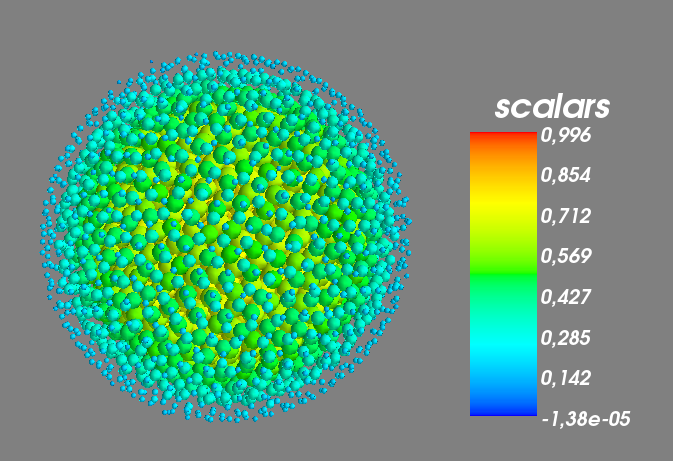
\includegraphics[scale=0.4]{images/mayavi3DPoints.png}
\caption{Plot with Mayavi. Mesh of a tetrahedron on a $3$D mesh with the solution on every vertex.}
\end{figure}

\subsection{Numerical results}
